\makeatletter%
\special{pdf: put @thispage <</Group << /S /Transparency /I true /CS /DeviceRGB>> >>}%
\makeatother%
\documentclass[a4paper,twoside,10pt]{article}
\usepackage[left=2.45cm,top=2.52cm,right=1.85cm,bottom=2.95cm]{geometry}

\usepackage[xetex]{hyperref}

\usepackage{csquotes}

\usepackage[printonlyused]{acronym}

\usepackage{graphicx}
\usepackage{caption}
\usepackage{subcaption}

\usepackage{booktabs}

\usepackage{amsmath}
\usepackage{txfonts}

\usepackage{minted}

\usepackage[backend=biber,style=alphabetic,natbib=true]{biblatex}
\addbibresource{bibliography.bib}

\title{Notes to Andrew Ng's Machine Learning Course}
\author{Jan Wedekind}

\begin{document}
\maketitle

\section{Introduction}

\subsection{What is Machine Learning}
These are course notes\footnote{source code here: \url{https://igit.comm.ad.roke.co.uk/jw4/machine-learning-tutorial}} to Andrew Ng's video lecture\citep{andrewng}.
A well-posed learning problem (as defined by Tom Mitchell) is:
\begin{displayquote}
  A computer program is said to \emph{learn} from experience E with respect to some task T and some performance measure P, if its performance on T, as measured by P, improves with experience E.
\end{displayquote}

\subsection{Supervised Learning}
\begin{figure}[htbp]
  \begin{center}
    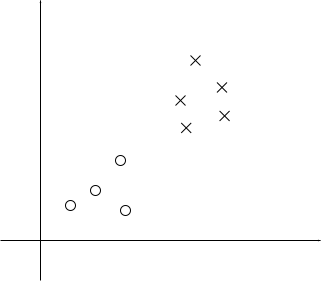
\includegraphics[width=.4\textwidth]{supervised}
    \caption{Labelled data for supervised learning\label{fig:supervised}}
  \end{center}
\end{figure}
Here are two examples for problems of different learning problems (given \emph{labelled} data as shown in Figure \ref{fig:supervised}):
\begin{itemize}
  \item Regression problem (\emph{continuous} value): estimating house price given size in square feet
  \item Classification problem (\emph{discrete} values): determine whether a tumor is malignant or benign given size of tumor and age of person
\end{itemize}

\subsection{Unsupervised Learning}
\begin{figure}[htbp]
  \begin{center}
    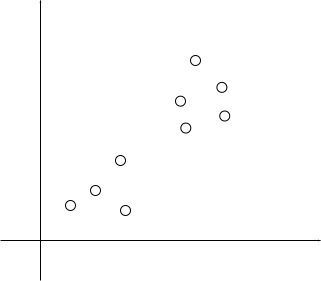
\includegraphics[width=.4\textwidth]{unsupervised}
    \caption{Data without labels\label{fig:unsupervised}}
  \end{center}
\end{figure}
When the data is not labelled (see \emph{unlabelled} data in Figure \ref{fig:unsupervised}), one can still apply clustering algorithms to it.
For example Google News clusters groups related news articles into stories.
Another basic but impressive example is separating two audio sources (speaker and a radio) using data from two microphones.

For development Andrew Ng recommends GNU Octave\citep{octave}.

\section{Linear Regression with One Variable}
\subsection{Model Representation}
\begin{table}[htbp]
  \begin{center}
    \begin{tabular}{r|r}\toprule
      \multicolumn{1}{c|}{\textbf{Size in feet$^2$ $(x)$}} &
      \multicolumn{1}{c}{\textbf{Price (\$) in 1000's $(y)$}}\\\midrule
      2104 & 460\\
      1416 & 232\\
      1534 & 315\\
       852 & 178\\
      $\vdots$ & $\vdots$\\\bottomrule
    \end{tabular}
    \caption{Table of house size and price\label{tbl:houses}}
  \end{center}
\end{table}
\newcommand{\sxi}{\ensuremath{x^{(i)}}}
\newcommand{\syi}{\ensuremath{y^{(i)}}}
\newcommand{\sumi}{\ensuremath{\displaystyle\sum_{i=1}^m}}
House price depending on house size example (see Table \ref{tbl:houses}): supervised regression problem.
The training set is denoted $(x,y)$ and the $i$th sample is $(\sxi,\syi)$ with $i\in\{1,2,\ldots,m\}$ where $m$ is the number of training samples.

The result of the learning algorithm is a \emph{hypothesis} $h$ which maps $x^\prime$ to an estimated value $y^\prime$.
\emph{E.g.} here the hypothesis is the linear function $h_\theta(x)=\theta_0+\theta_1\,x$.

Linear regression with one variable (the variable here is $x$) can also be called \emph{univariate} linear regression.

\subsection{Cost Function}\label{cha:costfunction}
The aim is to minimize the $h_\theta(x)-y$.
\emph{I.e.} minimizing the cost function (or square error function) $J(\theta_0,\theta_1)$ in the following equation
\begin{equation*}
  \displaystyle\mathop{\operatorname{argmin}}_{\theta_0,\theta_1}\underbrace{\frac{1}{2\,m}\,\sumi\big(h_\theta(\sxi)-\syi\big)^2}_{\eqqcolon J(\theta_0,\theta_1)}
\end{equation*}

\subsection{Cost Function Intuition}
With the simplified hypothesis $h_\theta(x)=\theta_1\,x$ we get
\begin{equation*}
  \theta_1=\mathop{\operatorname{argmin}}_{\theta_1}J(\theta_1)=\mathop{\operatorname{argmin}}_{\theta_1}\frac{1}{2\,m}\,\sumi\big(\theta_1\,\sxi-\syi\big)^2
\end{equation*}
The minimum can be obtained by solving for where the derivative is zero
\begin{equation*}
  \frac{\delta}{\delta\theta_1}J(\theta_1)=\frac{1}{m}\,\sumi\big(\theta_1\,\sxi-\syi\big)\,\sxi\overset{!}{=}0\Leftrightarrow
  \theta_1=\sumi\sxi\,\syi\bigg/\sumi\sxi\,\sxi
\end{equation*}
Using a contour plot one can visualise the two-dimensional version of $J(\theta_0,\theta_1)$ when using the full model.

Least-square estimation for $h_\theta(x)=\theta_0+\theta_1\,x$ yields
\begin{equation*}
\frac{1}{m}\,\sumi\big(\theta_0+\theta_1\,\sxi-\syi\big)\,\begin{pmatrix}1\\\sxi\end{pmatrix}\overset{!}{=}\vec{0}\Leftrightarrow
\begin{pmatrix}\theta_0\\\theta_1\end{pmatrix}=
\begin{pmatrix}m&\sum\sxi\\\sum\sxi&\sum\sxi\,\sxi\end{pmatrix}^{-1}\,
\begin{pmatrix}\sum\syi\\\sum\sxi\,\syi\end{pmatrix}
\end{equation*}
See Appendix \ref{app:lse} for the implementation. Figure \ref{fig:lse} shows sample data with a least square fit.
\begin{figure}[htbp]
  \begin{center}
    \includegraphics[width=.6\textwidth]{least_squares}
    \caption{Example data and corresponding least square fit of a linear function\label{fig:lse}}
  \end{center}
\end{figure}

\subsection{Gradient Descent}\label{cha:gradientdescent}
Starting from an initial solution $\theta_j$ with $j\in\{0,1\}$, the solution is updated iteratively using
\begin{equation*}
  \theta_j\coloneqq\theta_j-\alpha\,\frac{\delta}{\delta\theta_j}J(\theta_0,\theta_1)
\end{equation*}
where $\alpha$ is the learning rate.
Note that the parameters are updated ``simultaneously'' using the gradient vector $\delta J/\delta\theta$
\begin{equation}\label{equ:gradientdescent}
  \theta\coloneqq\theta-\alpha\,\frac{\delta}{\delta\theta}J(\theta)
\end{equation}

\subsection{Gradient Descent Intuition}
\begin{itemize}
  \item If $\alpha$ is too small, the algorithm will converge slowly.
  \item If $\alpha$ is too large, the algorithm will not converge on the local minimum.
\end{itemize}

\subsection{Gradient Descent for Linear Regression}
Gradient descent is performed using Equation (\ref{equ:gradientdescent}). Here the gradient is
\begin{equation*}
  \frac{\delta}{\delta\theta}J(\theta)=
  \frac{1}{m}\,\sumi\big(\theta_0+\theta_1\,\sxi-\syi\big)\,\begin{pmatrix}1\\\sxi\end{pmatrix}=
  \frac{1}{m}\,\begin{pmatrix}m&\sum\sxi\\\sum\sxi&\sum\sxi\,\sxi\end{pmatrix}\,
  \begin{pmatrix}\theta_0\\\theta_1\end{pmatrix}
\end{equation*}

See Appendix \ref{app:gradientdescent} for an implementation using symbolic differentiation of the cost function $J$.
A result of the iterative algorithm is shown in Figure \ref{fig:gradient_descent}.
\begin{figure}[htbp]
  \begin{center}
    \includegraphics[width=.6\textwidth]{gradient_descent}
    \caption{Example data and corresponding least square fit of a linear function\label{fig:gradient_descent}}
  \end{center}
\end{figure}

\section{Linear Regression with Multiple Variables}
\subsection{Multiple Features}
In the case of $n$ features, each feature $\sxi$ is a $n+1$ dimensional feature vector with $x_0$ set to $1$ for convenience:
\begin{equation*}
  \sxi=\begin{pmatrix}\sxi_0\\\sxi_1\\\vdots\\\sxi_n\end{pmatrix}\in\mathbb{R}^{n+1}
  \mathrm{\ where\ }\sxi_0\coloneqq 1
\end{equation*}
The hypothesis $h$ is
\begin{equation*}
  h_\theta(x)=\theta_0+\theta_1\,x_1+\theta_2\,x_2+\ldots+\theta_n\,x_n
\end{equation*}
Using $x_0=1$ the hypothesis can be written more compactly using the vector inner product:
\begin{equation*}
  h_\theta(x)=\theta^\top x
\end{equation*}
Regression using multiple variables is called \emph{multivariate regression}.

\subsection{Gradient Descent for Multiple Variables}\label{cha:linearregression}
The cost function $J$ can be written using vector notation
\begin{equation*}
  J(\theta)=\frac{1}{2\,m}\sumi\big(h_\theta(\sxi)-\syi\big)^2
\end{equation*}
As in Section \ref{cha:gradientdescent}, gradient descent is performed using the parameter $\alpha$:
\begin{equation*}
  \theta_j\coloneqq\theta_j-\alpha\cdot\underbrace{\frac{\delta}{\delta\theta_j}J(\theta)}_
  {\frac{1}{m}\sumi\big(h_\theta(\sxi)-\syi\big)\,\sxi}\mathrm{\ for\ }j\in\{0,\ldots,n\}
\end{equation*}

\subsection{Feature Scaling}
Feature scaling is about scaling $x_1,x_2,\ldots$ so that the variation of the values is similar.
Gradient descent then will converge more quickly (see Figure \ref{fig:scaling}).
\begin{figure}[htbp]
  \begin{center}
    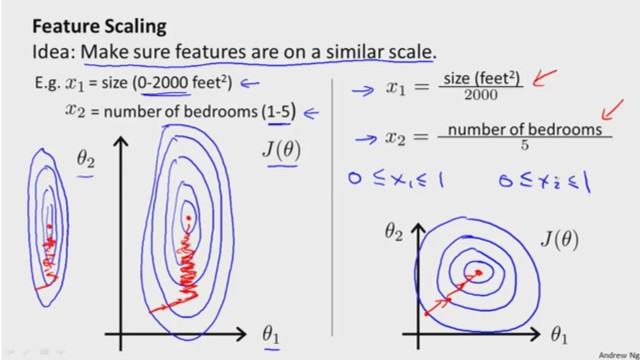
\includegraphics[width=.6\textwidth]{scaling}
    \caption{Feature scaling improves the performance of gradient descent\citep{andrewng}\label{fig:scaling}}
  \end{center}
\end{figure}
A common approach is to normalise the features to zero mean ($\mu=0$) and a standard deviation of one ($\sigma=1$).

\subsection{Learning Rate}
When performing gradient descent, $J(\theta)$ should decrease after each iteration.
Plotting $J(\theta)$ over each iteration can help to tell whether gradient descent has converged (see Figure \ref{fig:alphas}).
If $J(\theta)$ is increasing, $\alpha$ might be too large.
\begin{figure}[htbp]
  \begin{center}
    \includegraphics[width=.6\textwidth]{learning_rate}
  \caption{Plotting the cost function over the iterations can help choosing an appropriate value for the learning rate $\alpha$\label{fig:alphas}}
  \end{center}
\end{figure}

\subsection{Features and Polynomial Regression}\label{cha:polyregression}
Similar as in support vector machines one can perform linear regression on non-linear functions of features.
\emph{I.e.} given a feature $x$, one can generate additional features $x^2$, $\sqrt x$, $\ldots$.

\subsection{Normal Equation}
An analytical solution for the linear regression problem exists since the cost function is a quadratic function and
can be written as follows
\begin{equation*}
  J(\theta)=a\,\theta^2+b\,\theta+c
\end{equation*}
An analytical solution for minimizing $J$ can be found by solving the following equation system
\begin{equation*}
  \frac{\delta}{\delta\theta_j}J(\theta)=0
\end{equation*}
The least squares problem is written in the following form.
\begin{equation*}
  \underbrace{\begin{pmatrix}
1&x^{(1)}_1&x^{(1)}_2&\hdots&x^{(1)}_n\\
1&x^{(2)}_1&x^{(2)}_2&\hdots&x^{(2)}_n\\
\vdots&\vdots&\vdots&\ddots&\vdots\\
1&x^{(m)}_1&x^{(m)}_2&\hdots&x^{(m)}_n
  \end{pmatrix}}_{\coloneqq X}\,\theta=
\underbrace{\begin{pmatrix}y^{(1)}\\\vdots\\y^{(m)}\end{pmatrix}}_{y}+\epsilon
\end{equation*}
The solution is $\theta=(X^\top X)^{-1}X^\top y$.

\subsection{Normal Equation Non Invertibility}
There are two cases where the least square solution $\theta=(X^\top X)^{-1}X^\top y$ is not invertible
\begin{itemize}
  \item redundant (linear dependent) features
  \item too many features (\emph{e.g.} more features than data, $m\le n$)
    \begin{itemize}
      \item delete some features or
      \item use regularisation
    \end{itemize}
\end{itemize}
The closed solution is preferable if the number of features $n$ is small (see Figure \ref{fig:gcp}).
\begin{figure}[htbp]
  \begin{center}
    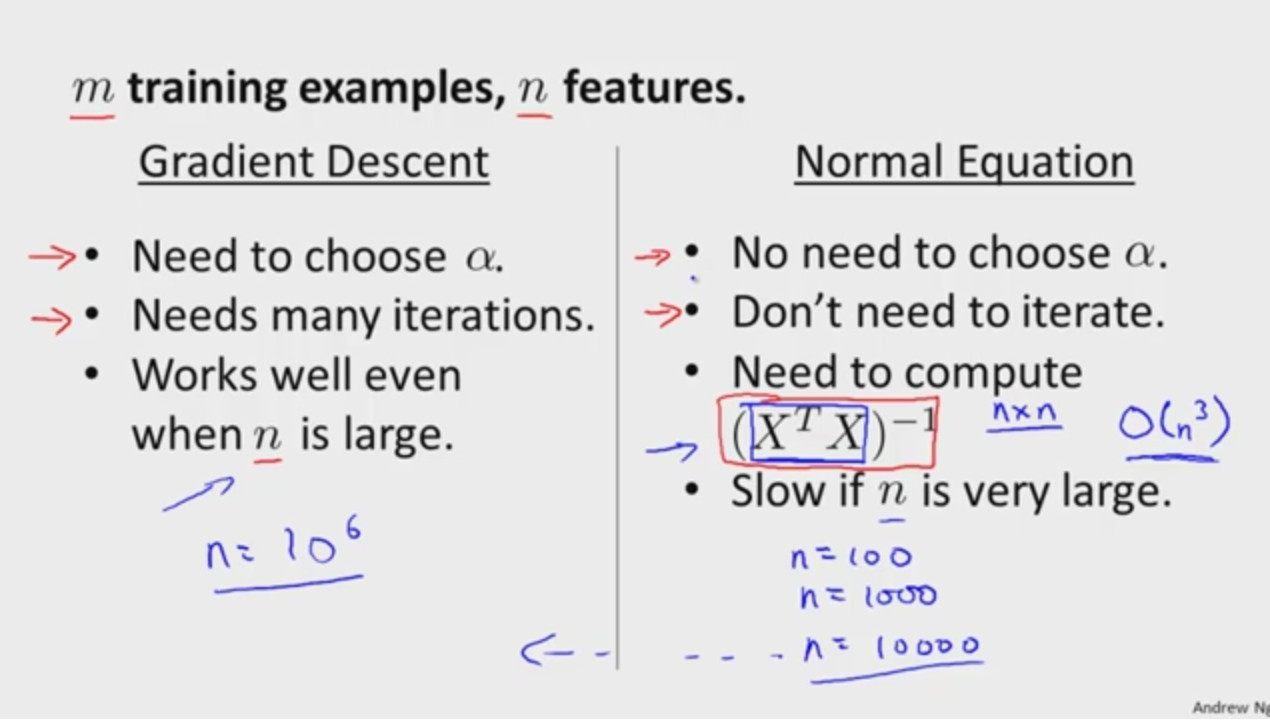
\includegraphics[width=.6\textwidth]{gradientproscons}
    \caption{Pros and cons for using gradient descent instead of the normal equation\citep{andrewng}\label{fig:gcp}}
  \end{center}
\end{figure}

\section{Logistic Regression}
\subsection{Classification}
The basic case is the binary classification problem $y\in\{0,1\}$.
Applying linear regression and thresholding the result (\emph{e.g.} $h_\theta(x)\ge 0.5$ generally does not perform well.
$0\le h_\theta(x)\le 1$ is not fullfilled for most linear models.

\subsection{Hypothesis Representation}
The logistic regression model uses the \emph{sigmoid} function (or \emph{logistic} function).
\begin{equation*}
  h_\theta(x)=g(\theta^\top x)\mathrm{\ where\ }g(z)=\frac{1}{1+\operatorname{e}^{-z}}
\end{equation*}
\begin{figure}[htbp]
  \begin{center}
    \includegraphics[width=.4\textwidth]{sigmoid}
    \caption{Sigmoid function\label{fig:sigmoid}}
  \end{center}
\end{figure}
Figure \ref{fig:sigmoid} shows the characteristic ``S''-shaped curve of the sigmoid function\footnote{\url{https://en.wikipedia.org/wiki/Sigmoid_function}}.
The model based on the sigmoid function is
\begin{equation*}
  h_\theta(x)=\frac{1}{1+\operatorname{e}^{-\theta^\top x}}
\end{equation*}
The output of $h_\theta(x)$ is interpreted as the estimated probability that $y=1$ on input $x$.
\begin{equation*}
  h_\theta(x)=P(y=1|\,x;\theta)
\end{equation*}

\subsection{Decision Boundary}
The prediction is
\begin{itemize}
  \item ``$y=1$'' if $h_\theta(x)\ge 0.5$
  \item ``$y=0$'' if $h_\theta(x)<0.5$
\end{itemize}
With $h_\theta(x)=g(\theta^\top x)$ and $g$ being monotonous, this is equivalent to
\begin{itemize}
  \item ``$y=1$'' if $\theta^\top x\ge 0$
  \item ``$y=0$'' if $\theta^\top x< 0$
\end{itemize}
The decision boundary in this case is a hyperplane in the feature space. \emph{E.g.} given two features
\begin{equation*}
  h_\theta(x)=g(\theta_0+\theta_1\,x_1+\theta_2\,x_2)
\end{equation*}
the decision boundary is
\begin{equation*}
  \theta_0+\theta_1\,x_1+\theta_2\,x_2=0
\end{equation*}
\begin{figure}[htbp]
  \begin{center}
    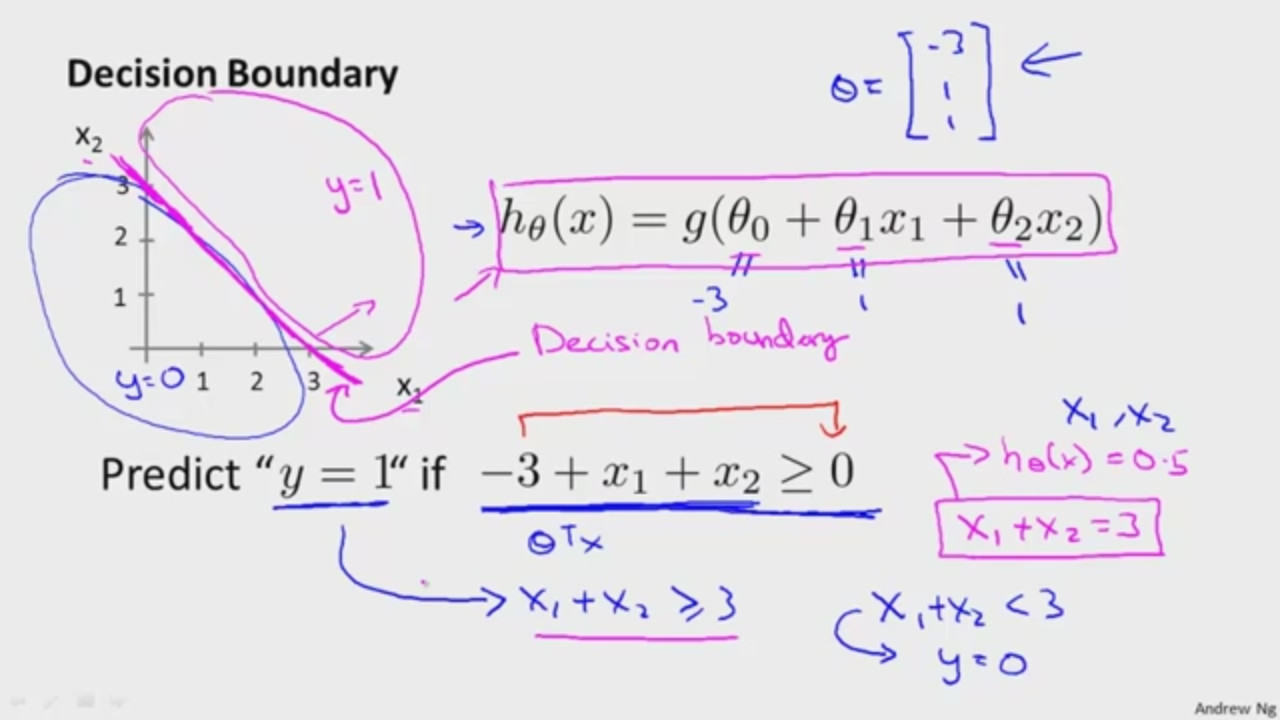
\includegraphics[width=.6\textwidth]{decisionboundary}
    \caption[Linear decision boundary]{Linear decision boundary. ``x'' denotes a positive sample (y=1) and ''o'' a negative sample (y=1)\label{fig:decisionboundary}}
  \end{center}
\end{figure}
It separates the ``y=1'' region and the ``y=0'' region (also see Figure \ref{fig:decisionboundary}).

\begin{figure}[htbp]
  \begin{center}
    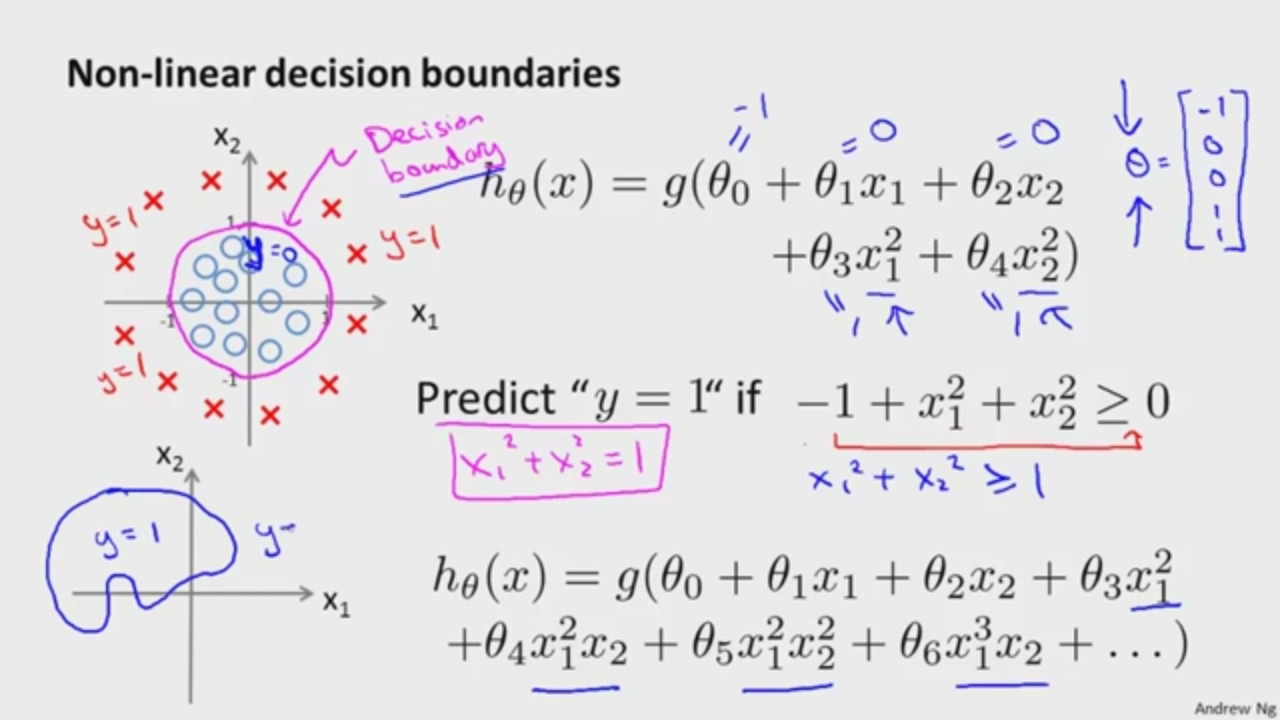
\includegraphics[width=.6\textwidth]{circularboundary}
    \caption{Circular decision boundary\label{fig:circularboundary}}
  \end{center}
\end{figure}
Similar as in Section \ref{cha:polyregression} one can use polynomial terms to introduce additional features in order to achieve a non-linear decision boundary (see Figure \ref{fig:circularboundary}). \emph{E.g.} one can use a circular decision boundary in the hypothesis
\begin{equation*}
  h_\theta(x)=g(\underbrace{\theta_0}_{=-1}+\underbrace{\theta_1}_{=0}\,x_1+\underbrace{\theta_2}_{=0}\,x_2+\underbrace{\theta_3}_{=1}\,x_1^2+\underbrace{\theta_4}_{=1}\,x_2^2)
\end{equation*}

\subsection{Cost Function}
Given
\begin{itemize}
\item a training set of $m$ training examples $\{(x^{(1)},y^{(1)},x^{(2)},y^{(2)},\ldots,x^{(m)},y^{(m)}\}$ with
$x\in\begin{pmatrix}x_0\\x_1\\\vdots\\x_n\end{pmatrix}$, $x_0=1$, $y\in\{0,1\}$
\item a hypothesis $h_\theta(x)=\displaystyle\frac{1}{1+\operatorname{e}^{-\theta^\top x}}$
\end{itemize}
Desired is a parameter vector $\theta$ so that $h_\theta(x)$ produces good predictions.

The cost function introduced in Section \ref{cha:costfunction} is generalised as follows
\begin{equation*}
  J(\theta)=\frac{1}{m}\sumi Cost(h_\theta(\sxi),\syi)
\end{equation*}
In the case of linear regression the cost function is $cost(h_\theta(x),y)=\frac{1}{2}(h_\theta(x)-y)^2$.
In the case of logistic regression this function would be ``non-convex''. Instead the following cost function is used
\begin{equation*}
Cost(h_\theta(x),y)=
\left\{\begin{array}{rl}-\operatorname{log}(h_\theta(x))&\mathrm{if\ }y=1\\
-\operatorname{log}(1-h_\theta(x))&\mathrm{if\ }y=0\end{array}\right.
\end{equation*}
\begin{figure}[htbp]
  \begin{center}
    \begin{subfigure}[b]{.47\textwidth}
      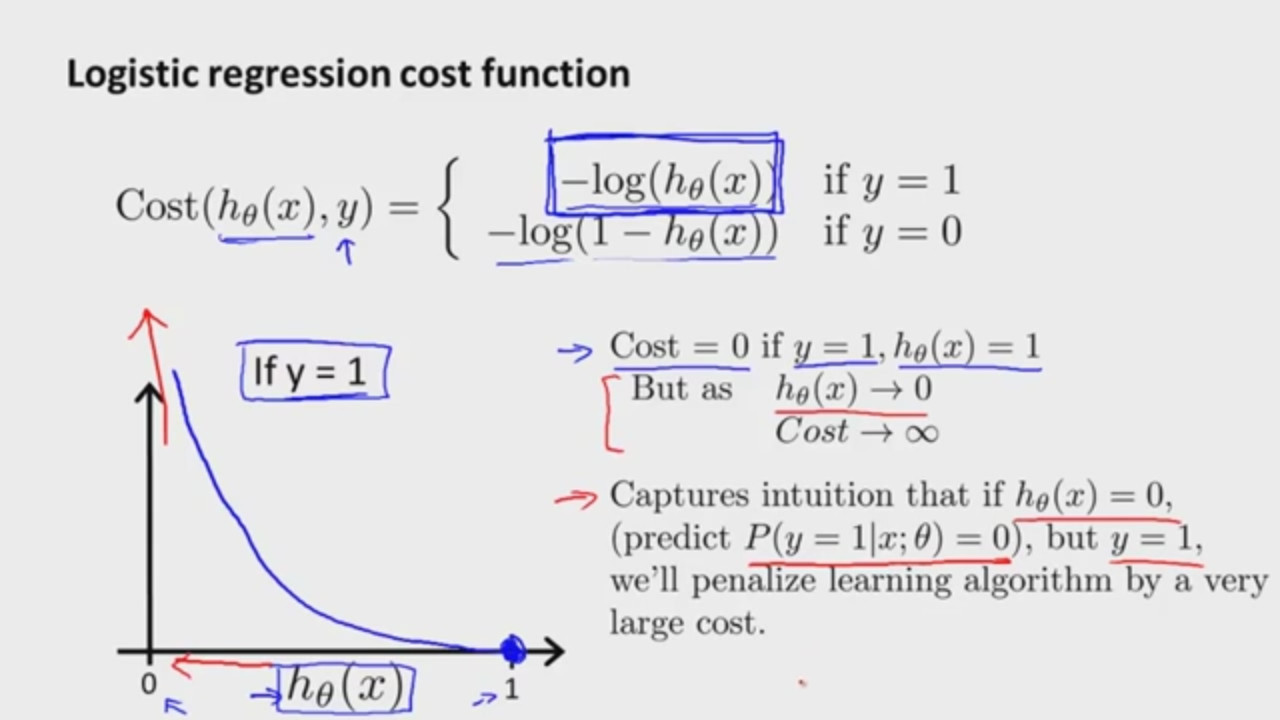
\includegraphics[width=\linewidth]{costy1}
      \caption{Cost function for ``y=1''}
    \end{subfigure}
    \begin{subfigure}[b]{.47\textwidth}
      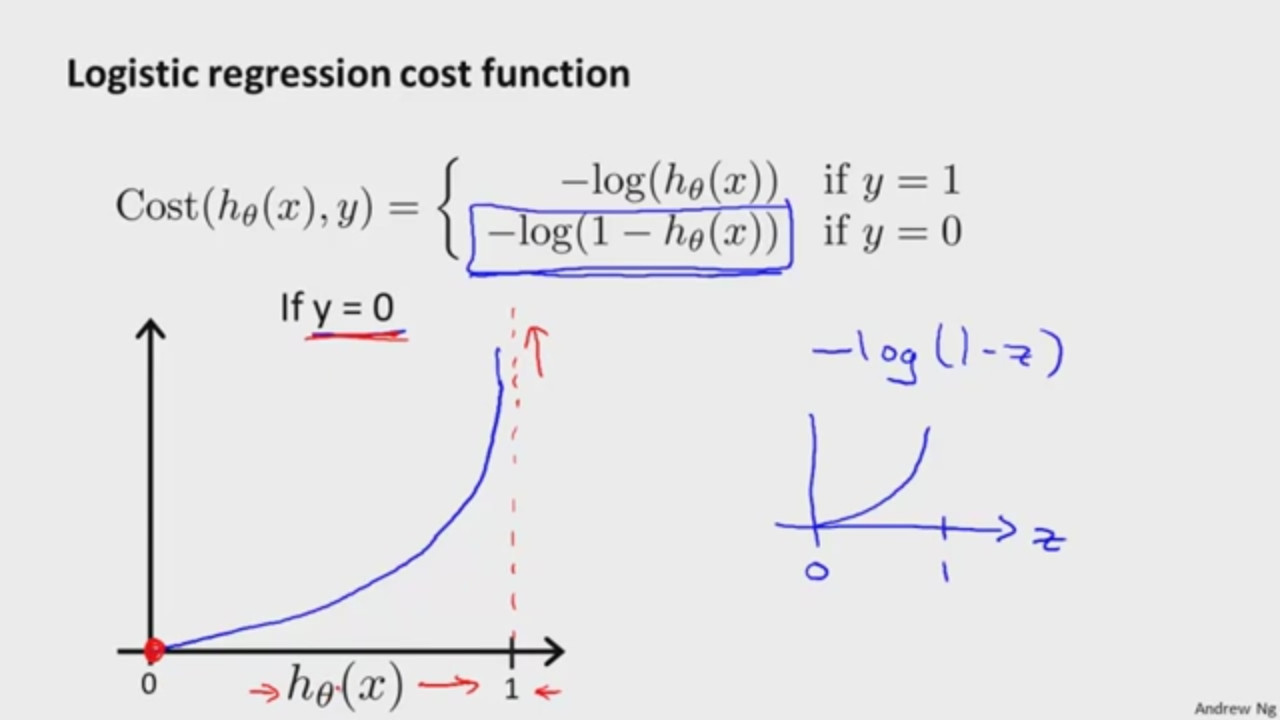
\includegraphics[width=\linewidth]{costy0}
      \caption{Cost function for ``y=0''}
    \end{subfigure}
    \caption{Cost function for logistic regression\label{fig:costlog}}
  \end{center}
\end{figure}
See Figure \ref{fig:costlog} for a visualisation.

\subsection{Simplified Cost Function and Gradient Descent}
The cost function
\begin{equation*}
Cost\big(h_\theta(x),y\big)=
\left\{\begin{array}{rl}-\operatorname{log}\big(h_\theta(x)\big)&\mathrm{if\ }y=1\\
-\operatorname{log}\big(1-h_\theta(x)\big)&\mathrm{if\ }y=0\end{array}\right.
\end{equation*}
can be rewritten as follows
\begin{equation*}
Cost\big(h_\theta(x),y\big)=
-y\,\operatorname{log}\big(h_\theta(x)\big)-(1-y)\,\operatorname{log}\big(1-h_\theta(x)\big)
\end{equation*}
The overall cost function $J(\theta)$ is\footnote{similar as in maximum likelihood estimation}
\begin{equation*}
  J(\theta)=-\frac{1}{m}\big[\sumi\syi\operatorname{log}h_\theta(\sxi)+(1-\syi)\operatorname{log}(1-h_\theta(\sxi))\big]
\end{equation*}

The minimization problem $\mathop{\operatorname{argmin}}_\theta J(\theta)$ can be solved using gradient descent
\begin{equation*}
  \theta_j\coloneqq\theta_j-\alpha\cdot\underbrace{\frac{\delta}{\delta\theta_j}J(\theta)}_
  {=\frac{1}{m}\sumi\big(h_\theta(\sxi)-\syi\big)\,\sxi}
\end{equation*}
Note that the choice of $h_\theta(x)=\frac{1}{1+\operatorname{e}^{-\theta^\top x}}$ for logistic regression has led to the \emph{same} gradient descent rule as used for linear regression (with $h_\theta(x)=\theta^\top x$ as shown in Section \ref{cha:linearregression}).

See Figure \ref{fig:classifier} for an example of classifying binary data with two features.
The corresponding implementation is shown in Appendix \ref{app:classifier}.
\begin{figure}[htbp]
  \begin{center}
    \includegraphics[width=.6\textwidth]{classifier}
    \caption{Classifying binary data with two features\label{fig:classifier}}
  \end{center}
\end{figure}

\subsection{Advanced Optimization}
There are other algorithms for optimizing the cost functions given
\begin{itemize}
  \item the cost function $J(\theta)$
  \item the derivative $\frac{\delta}{\delta\theta_j}J(\theta)$
\end{itemize}
Some optimization algorithms are
\begin{itemize}
  \item Gradient descent
  \item Conjugate gradient
  \item \acs{BFGS}\footnote{\url{https://en.wikipedia.org/wiki/Broyden\%E2\%80\%93Fletcher\%E2\%80\%93Goldfarb\%E2\%80\%93Shanno_algorithm}}
  \item \acs{L-BFGS}\footnote{\url{https://en.wikipedia.org/wiki/Limited-memory_BFGS}}
\end{itemize}
More advanced algorithms have the following advantages
\begin{itemize}
  \item no need to manually pick $\alpha$
  \item often converge faster than gradient descent
\end{itemize}
However the algorithms are more complex. It is not recommended to implement this algorithms yourself.

\subsection{MultiClass Classification: One-vs-all}
The binary classifier can be generalised to multiclass problems using multiple one-vs-all classifiers.
\emph{E.g.} for $y\in\{1,2,3\}$ three classifiers $h_\theta^{(i)}(x)=P(y=i\|\,x;\theta)$ for $i\in\{1,2,3\}$ are trained.
To make a prediction, the classifier outputting the highest probability is selected (see Figure \ref{fig:onevsall}):
\begin{equation*}
  \mathop{\operatorname{max}}_ih_\theta^{(i)}(x)
\end{equation*}
\begin{figure}[htbp]
  \begin{center}
    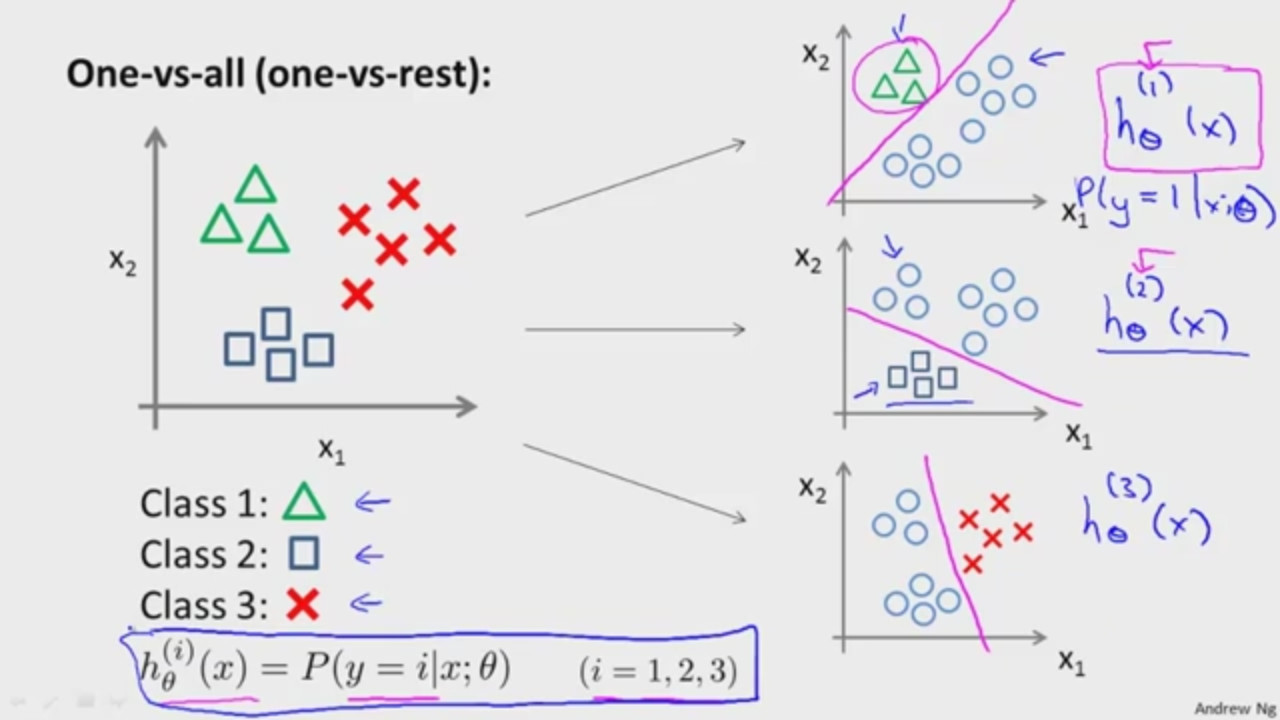
\includegraphics[width=.6\textwidth]{onevsall}
    \caption{Multiclass classification using one-vs-all classifiers\label{fig:onevsall}}
  \end{center}
\end{figure}

\clearpage

\appendix
\section{Appendix}
\subsection{Least Squares Estimator}\label{app:lse}
\inputminted[frame=lines,linenos,fontsize=\small]{python}{least_squares.py}

\subsection{Linear Regression}\label{app:gradientdescent}
\inputminted[frame=lines,linenos,fontsize=\small]{python}{gradient_descent.py}

\subsection{Learning Rate}\label{app:alphas}
\inputminted[frame=lines,linenos,fontsize=\small]{python}{learning_rate.py}

\subsection{Logistic Regression}\label{app:classifier}
\inputminted[frame=lines,linenos,fontsize=\small]{python}{classifier.py}

\subsection{Convolution using Theano}
\inputminted[frame=lines,linenos,fontsize=\small]{python}{convolution.py}

\section{References and Glossary}
\subsection{References}
\printbibliography[heading=none]

\subsection{Glossary}
\begin{acronym}[L-BFGS]
  \acro{BFGS}{Broyden-Fletcher-Goldfarb-Shanno algorithm}
  \acro{L-BFGS}{Limited-memory BFGS}
\end{acronym}

\end{document}
